\documentclass[11pt]{article}

% ---------- layout & fonts ----------
\usepackage[margin=1in]{geometry}
\usepackage[T1]{fontenc}
\usepackage[utf8]{inputenc}
\usepackage{XCharter}                 % clean, readable text font
\usepackage[xcharter]{newtxmath}      % matching math font
\usepackage{microtype}
\usepackage[varqu]{zi4}               % clean monospace font (Inconsolata)
\usepackage{graphicx}
\usepackage{booktabs}
\usepackage{amsmath}
\usepackage{xcolor}
\usepackage[round]{natbib}
\usepackage[colorlinks=true, linkcolor={blue!50!black}, citecolor={blue!50!black}, urlcolor={blue!50!black}]{hyperref}
\usepackage[font=small, labelfont=bf]{caption}
\usepackage[section]{placeins}   % keeps figures/tables inside their own section

\setlength{\parindent}{0pt}
\setlength{\parskip}{0.6em}

% Boxes for the full prompt text (Appendix A)
\usepackage[most]{tcolorbox}
\newtcolorbox{promptbox}[1]{enhanced, breakable, before skip=0.8em, after skip=0.8em,
  colback=gray!4, colframe=gray!45, boxrule=0.5pt, arc=2pt,
  left=10pt, right=10pt, top=8pt, bottom=8pt,
  colbacktitle=gray!14, coltitle=black, fonttitle=\bfseries\small, title={#1},
  fontupper=\small\ttfamily\raggedright\frenchspacing, parbox=false, before upper={\setlength{\parskip}{0.7em}}}
\newcommand{\slot}[1]{\textcolor{blue!55!black}{\texttt{\{#1\}}}}

% Anything in \fillme{...} still needs your input (shows up red in the PDF).
\newcommand{\fillme}[1]{\textcolor{red}{[#1]}}

\title{\textbf{Can Small Language Models Review Research Papers?}\\[0.3em]
\large A Pilot Study on ICLR 2024 Submissions}
\author{Pawan Chaudhary\\ \small Independent Researcher}
\date{October 2026}

\begin{document}
\maketitle

% =====================================================================
\begin{abstract}
\noindent
Large language models (LLMs) are starting to be used as reviewers of research papers. Before trusting one, we should know whether its verdict depends on the paper or on how the question is asked. I tested three small open models (Qwen2.5 with 1.5, 3, and 7 billion parameters) on 60 papers submitted to ICLR 2024, half accepted and half rejected. Each model rated each paper four times, using four prompts that ask the same question in different words. I found three problems. First, the models are far too generous: every model gave a passing score to every paper. Second, the verdict depends on the wording: 18--33\% of papers are accepted under one prompt and rejected under another. Third, the models barely agree with human reviewers: their scores have little relationship with the reviewers' ratings, and even the largest model separates accepted from rejected papers only moderately well. A single prompt to a small LLM is therefore not a reliable paper review. All code and data are released.
\end{abstract}

% =====================================================================
\section{Introduction}

LLMs are now often used to judge the output of other models, and strong models agree with human judges about as often as humans agree with each other \citep{zheng2023judging}. The same idea is being applied to science. The AI Scientist \citep{lu2024aiscientist} writes complete research papers and uses an LLM reviewer to decide which ones are good, and \citet{liang2023feedback} study whether LLM feedback on real papers is useful. If the reviewer is unreliable, everything built on top of it is unreliable too.

There is good reason to be careful. LLM judges can be swayed by details that should not matter, such as which answer is shown first or which one is longer \citep{zheng2023judging}, and small changes to how a prompt is formatted can change an LLM's answers a lot \citep{sclar2023quantifying, mizrahi2024state}. Most work on LLM reviewers uses large commercial models and a single fixed prompt. Much less is known about small open models, which are the ones students and small labs can actually run.

This paper asks two simple questions:
\begin{enumerate}
  \item If a small LLM rates the same paper using prompts that mean the same thing, does it give the same verdict?
  \item Does its verdict agree with human reviewers?
\end{enumerate}

The short answer to both is: not reliably. In more detail:
\begin{itemize}
  \item \textbf{Too generous.} All three models gave a passing score (6 or more out of 10) to 100\% of papers, although only half were accepted.
  \item \textbf{Sensitive to wording.} Between 18\% and 33\% of papers switch between accept and reject depending only on the prompt.
  \item \textbf{Out of step with humans.} Model scores are only weakly related to human ratings. Larger models do somewhat better, but not by much.
\end{itemize}

% =====================================================================
\section{Related Work}

\textbf{LLMs as judges and reviewers.}
\citet{zheng2023judging} found that GPT-4 agrees with human preferences over 80\% of the time, as often as humans agree with each other, but also that it favors answers shown first and answers that are longer. The AI Scientist \citep{lu2024aiscientist} built an LLM reviewer that follows conference reviewing guidelines and reported accuracy close to human reviewers on ICLR 2022 papers. \citet{liang2023feedback} found that GPT-4's comments on research papers overlap with human reviewers' comments about as much as two human reviewers overlap with each other. All of these use large commercial models and one prompt.

\textbf{Sensitivity to prompts.}
\citet{sclar2023quantifying} showed that formatting changes that do not change a prompt's meaning can cause large swings in LLM accuracy, and \citet{mizrahi2024state} argue that results should be reported across many versions of a prompt, not just one. This paper applies that idea to paper reviewing, with small models.

% =====================================================================
\section{Method}

\subsection{Papers}
I used 60 papers submitted to ICLR 2024, a major machine learning conference: 30 accepted and 30 rejected, picked at random from papers with at least three reviews. ICLR publishes its reviews on OpenReview; I used a copy of them hosted on Hugging Face (\texttt{smallari/\allowbreak openreview-\allowbreak iclr2024-\allowbreak peer-\allowbreak reviews-\allowbreak RAW}). The models saw only each paper's title and abstract. For comparison I used the real decision and the average reviewer rating. Accepted papers had an average rating of 6.37 out of 10; rejected papers had 4.62.

\subsection{Models}
I used three sizes of the Qwen2.5 model family \citep{qwen2024qwen25}: 1.5, 3, and 7 billion parameters. All three are free and open, and I ran them on free Kaggle GPUs.

\subsection{Prompts}
I wrote four prompts that all ask for the same thing: an overall score for the paper from 1 (reject) to 10 (accept), answered with a single number. They differ only in details that should not matter (Table~\ref{tab:prompts}; full text in Appendix~\ref{app:prompts}). A good reviewer should give the same score whichever prompt it gets.

\begin{table}[!htbp]
\centering
\begin{tabular}{ll}
\toprule
\textbf{Prompt} & \textbf{How it differs} \\
\midrule
P1 (expert) & Tells the model it is an expert reviewer; instructions come first \\
P2 (plain)  & Plain description of the task, no role \\
P3 (after)  & Instructions come \emph{after} the paper instead of before \\
P4 (terse)  & Very short, with markdown headings \\
\bottomrule
\end{tabular}
\caption{The four prompts. All ask for the same 1--10 score.}
\label{tab:prompts}
\end{table}

\subsection{Scores}
For each rating I recorded two numbers. The first is simply the score the model writes. This turned out to be almost always 8, which makes differences hard to see. So I also used a finer score: the model's average answer, weighted by how likely it considers each score from 1 to 10. For example, a model that is 70\% sure of 8 and 30\% sure of 7 gets a finer score of 7.7. Technical details are in Appendix~\ref{app:details}.

\subsection{What I measured}
\begin{itemize}
  \item \textbf{Generosity:} the share of ratings with a written score of 6 or more, which on ICLR's scale leans toward acceptance.
  \item \textbf{Consistency across prompts:} how often a paper's verdict changes with the prompt. Under each prompt, the top 31\% of papers by finer score count as accepted, matching ICLR 2024's real acceptance rate. A paper \emph{flips} if it is accepted under one prompt and rejected under another. If the models ranked papers at random, about 76\% of papers would flip.
  \item \textbf{Agreement with humans:} two standard measures. The \emph{correlation} with the average human rating runs from 0 (no relationship) to 1 (the model ranks papers exactly like the humans). The \emph{AUC} measures how well the score separates accepted from rejected papers: 0.5 is a coin flip, 1 is perfect.
\end{itemize}
With only 60 papers, every number has some uncertainty. Where I give a range in brackets, it is a 95\% confidence interval: the range the true value most likely falls in.

% =====================================================================
\section{Results}

\begin{table}[!htbp]
\centering
\small
\begin{tabular}{lcccc}
\toprule
\textbf{Model} & \textbf{Most common} & \textbf{Passing score} & \textbf{Prompts agree} & \textbf{Papers that flip} \\
 & \textbf{written score} & \textbf{(6 or more)} & \textbf{on ranking} & \textbf{(random would be 76\%)} \\
\midrule
Qwen2.5 1.5B & 8 (71\% of ratings) & 100\% & 0.80 & 27\% \\
Qwen2.5 3B   & 8 (86\% of ratings) & 100\% & 0.77 & 33\% \\
Qwen2.5 7B   & 8 (69\% of ratings) & 100\% & 0.80 & 18\% \\
\bottomrule
\end{tabular}
\caption{Generosity and consistency. ``Prompts agree on ranking'' is the average correlation between the rankings that two different prompts produce (1 = identical).}
\label{tab:stability}
\end{table}

\subsection{The models are far too generous}
\label{sec:leniency}
The models give almost every paper an 8, and every model gives a passing score to 100\% of papers, even though only half were accepted (Table~\ref{tab:stability}). A reviewer that accepts everything is not really reviewing. This also hides a second problem: if you only look at pass or fail, the models look perfectly consistent across prompts, but only because they never say no.

I can only guess at the cause. These models are trained to be helpful and agreeable, and abstracts are written to sell the paper and rarely mention its weaknesses. Both would push toward a generous score.

\subsection{The verdict depends on the wording}
The finer score shows what the written score hides. The four prompts mostly agree on which papers are better than others (agreement around 0.8), so the models are not random. But when each prompt accepts its top 31\%, between 18\% (7B) and 33\% (3B) of papers are accepted under one prompt and rejected under another. That is far better than random (76\%), but it still means roughly one paper in four or five has its fate decided by the wording of the prompt rather than its content.

The prompt also shifts the scores as a whole. Just by changing the prompt, the average score moved by up to 0.84 points out of 10 (for the 3B model). Since most scores sit in a narrow band between about 7.5 and 9 (Figure~\ref{fig:spread}), a shift this large means any fixed cut-off for acceptance would depend on which prompt was used.

\begin{figure}[!htbp]
\centering
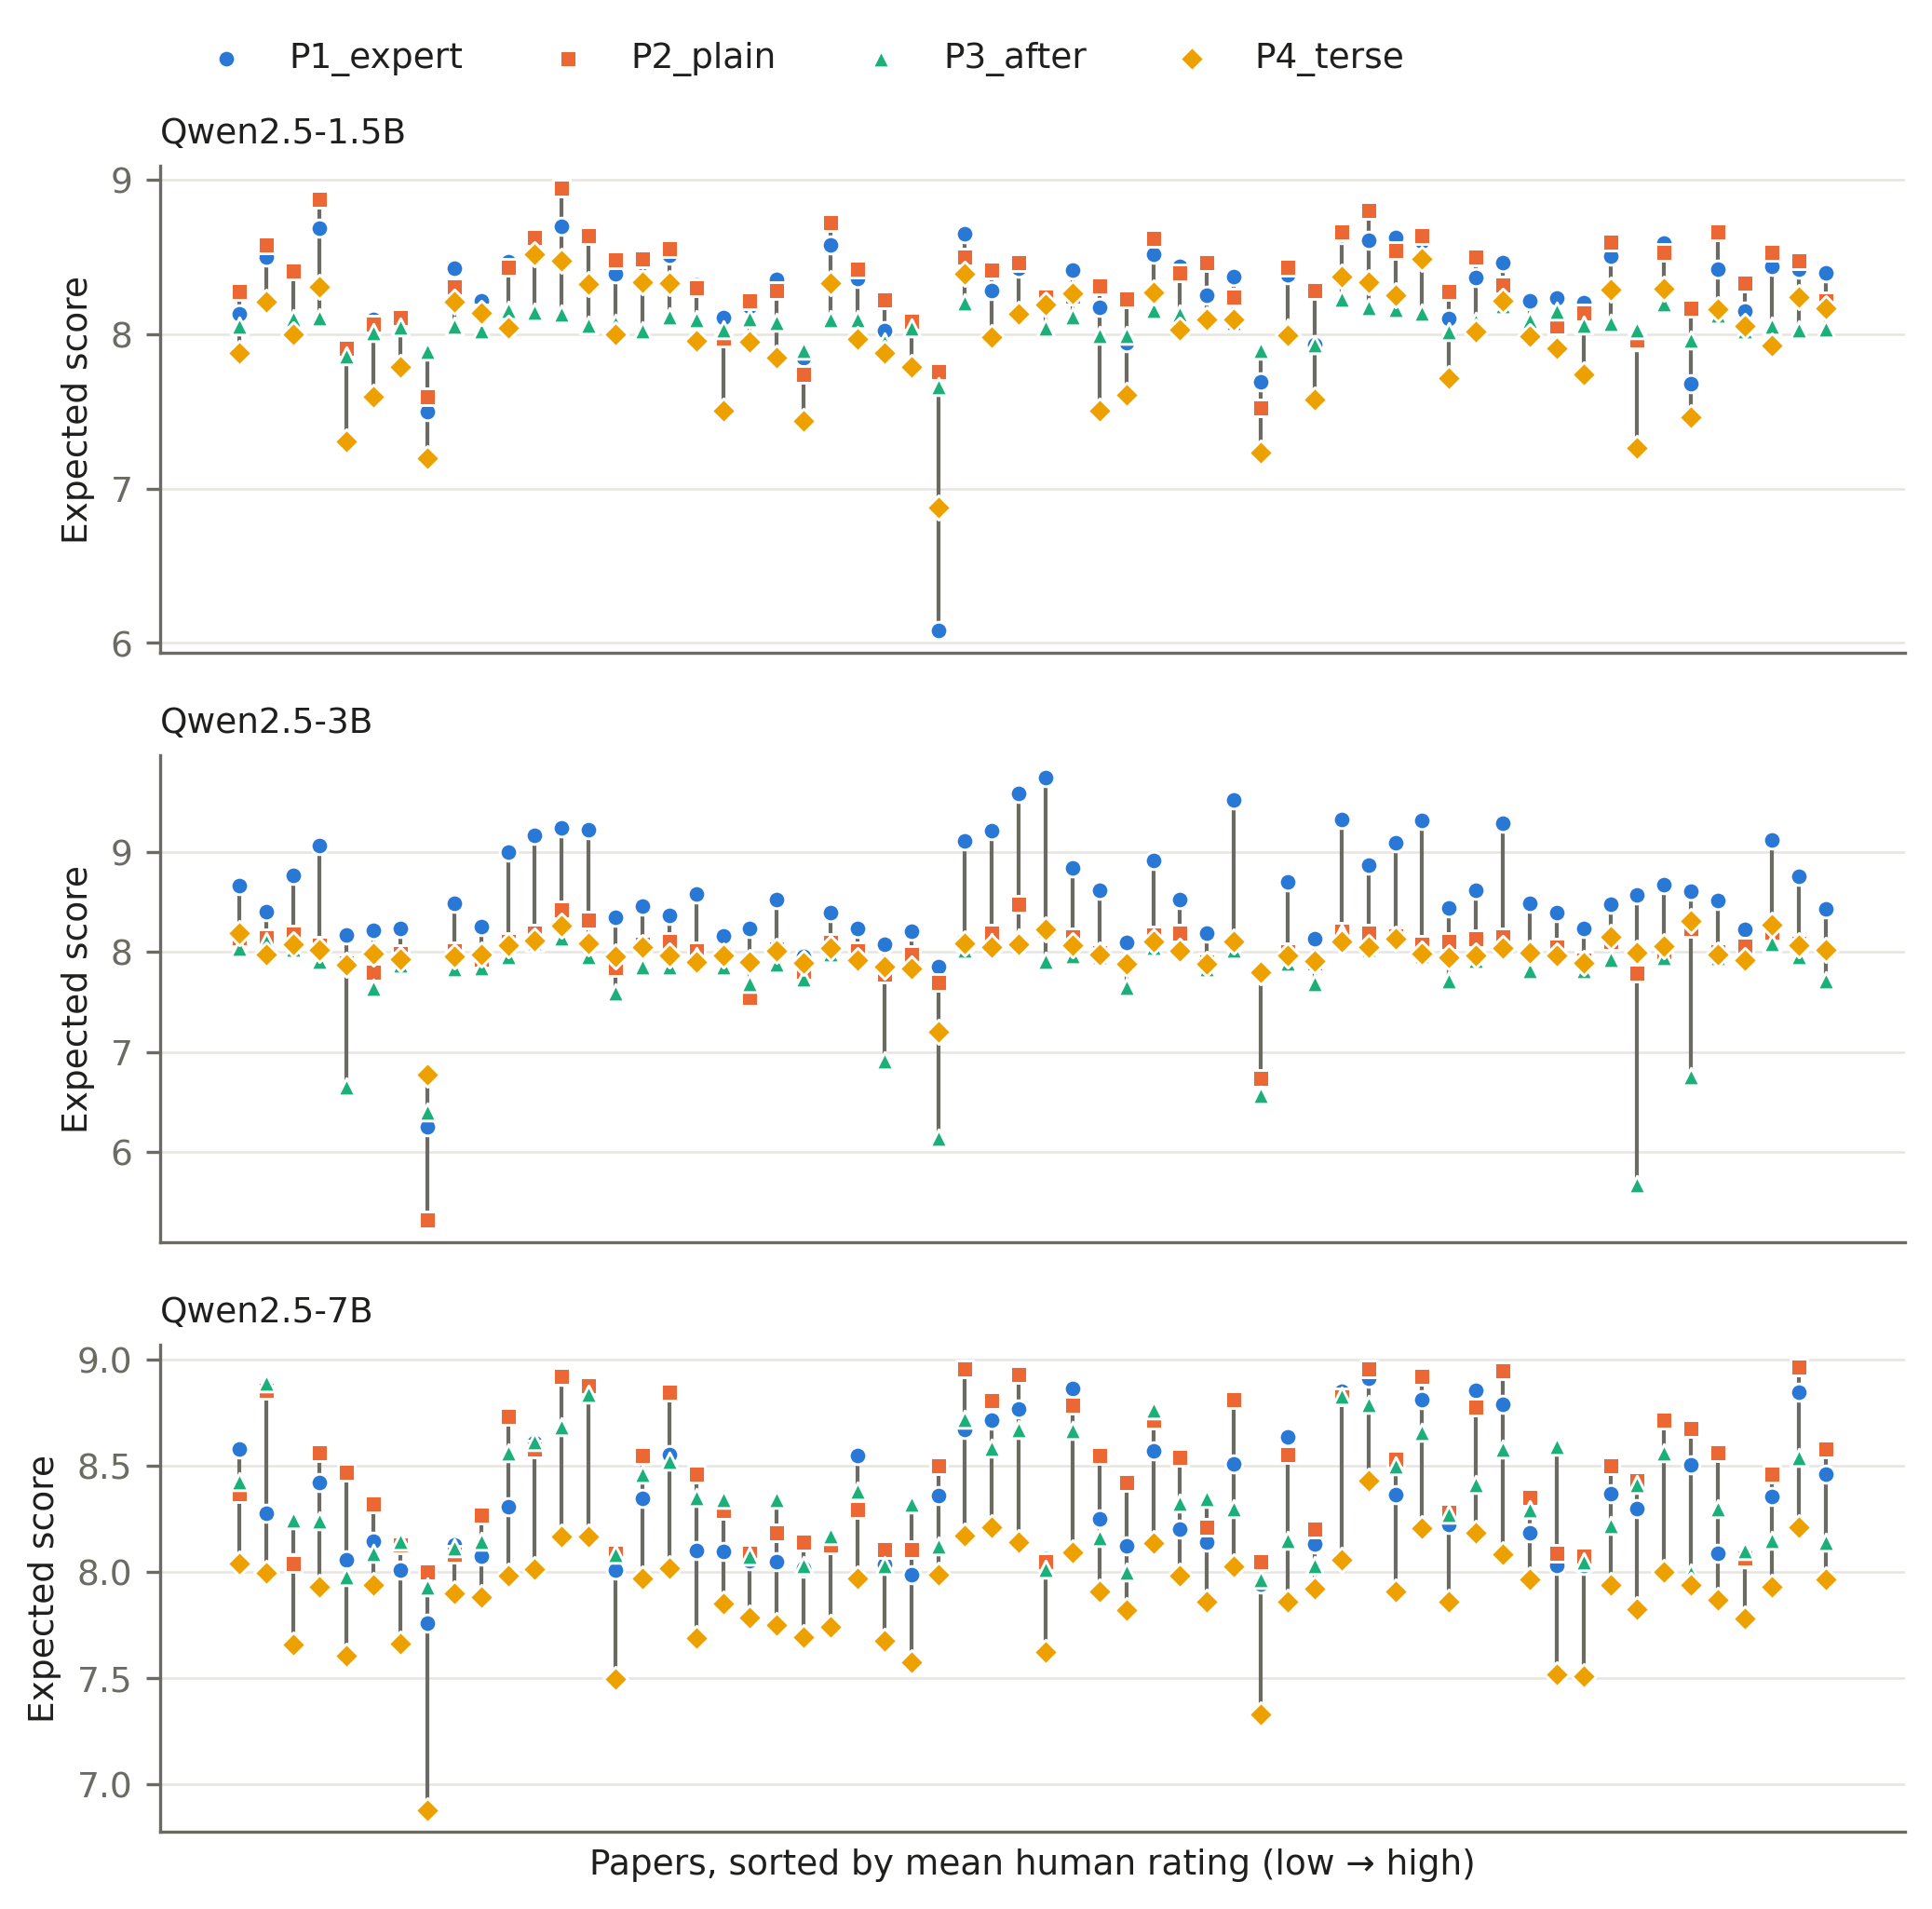
\includegraphics[width=0.92\textwidth]{figures/fig1_score_spread.png}
\caption{Each column is one paper; the four markers are its finer scores (``expected score) under the four prompts, and the gray line spans the lowest to the highest. Papers are sorted from lowest to highest human rating. If the models agreed with humans, scores would rise from left to right; they barely do.}
\label{fig:spread}
\end{figure}

\subsection{The models barely agree with human reviewers}
The correlation between model scores and human ratings is between 0.01 and 0.24 (Table~\ref{tab:agreement}, Figure~\ref{fig:agreement}), which is weak. For almost every model and prompt, the confidence interval includes zero, so we cannot rule out that there is no relationship at all. Telling accepted papers apart from rejected ones works a little better and improves with model size: the AUC is about 0.60 for the 1.5B model and about 0.70 for the 7B model, where it is clearly better than a coin flip. So the largest model picks up a rough accept-or-reject signal, but it does not rank papers the way human reviewers do.

\begin{table}[!htbp]
\centering
\begin{tabular}{llcc}
\toprule
\textbf{Model} & \textbf{Prompt} & \textbf{Correlation with humans} & \textbf{AUC (accepted vs.\ rejected)} \\
\midrule
1.5B & P1 expert & 0.01 \small[$-$0.27, 0.27] & 0.60 \small[0.46, 0.74] \\
     & P2 plain  & 0.05 \small[$-$0.21, 0.32] & 0.58 \small[0.42, 0.72] \\
     & P3 after  & 0.05 \small[$-$0.19, 0.28] & 0.64 \small[0.49, 0.77] \\
     & P4 terse  & 0.04 \small[$-$0.20, 0.29] & 0.60 \small[0.46, 0.74] \\
     & Average of all four & 0.03 \small[$-$0.24, 0.29] & 0.61 \small[0.47, 0.75] \\
\midrule
3B   & P1 expert & 0.16 \small[$-$0.05, 0.37] & 0.66 \small[0.52, 0.80] \\
     & P2 plain  & 0.13 \small[$-$0.13, 0.37] & 0.58 \small[0.42, 0.73] \\
     & P3 after  & 0.04 \small[$-$0.20, 0.30] & 0.67 \small[0.52, 0.81] \\
     & P4 terse  & 0.15 \small[$-$0.11, 0.39] & 0.58 \small[0.43, 0.73] \\
     & Average of all four & 0.09 \small[$-$0.15, 0.32] & 0.64 \small[0.50, 0.78] \\
\midrule
7B   & P1 expert & 0.24 \small[0.01, 0.45] & 0.70 \small[0.56, 0.83] \\
     & P2 plain  & 0.19 \small[$-$0.06, 0.41] & 0.70 \small[0.56, 0.83] \\
     & P3 after  & 0.03 \small[$-$0.23, 0.30] & 0.68 \small[0.53, 0.80] \\
     & P4 terse  & 0.15 \small[$-$0.09, 0.39] & 0.69 \small[0.55, 0.81] \\
     & Average of all four & 0.17 \small[$-$0.08, 0.39] & 0.70 \small[0.57, 0.82] \\
\bottomrule
\end{tabular}
\caption{Agreement with human reviewers, with 95\% confidence intervals in brackets. Correlation: 0 = no relationship. AUC: 0.5 = coin flip.}
\label{tab:agreement}
\end{table}

\begin{figure}[!htbp]
\centering
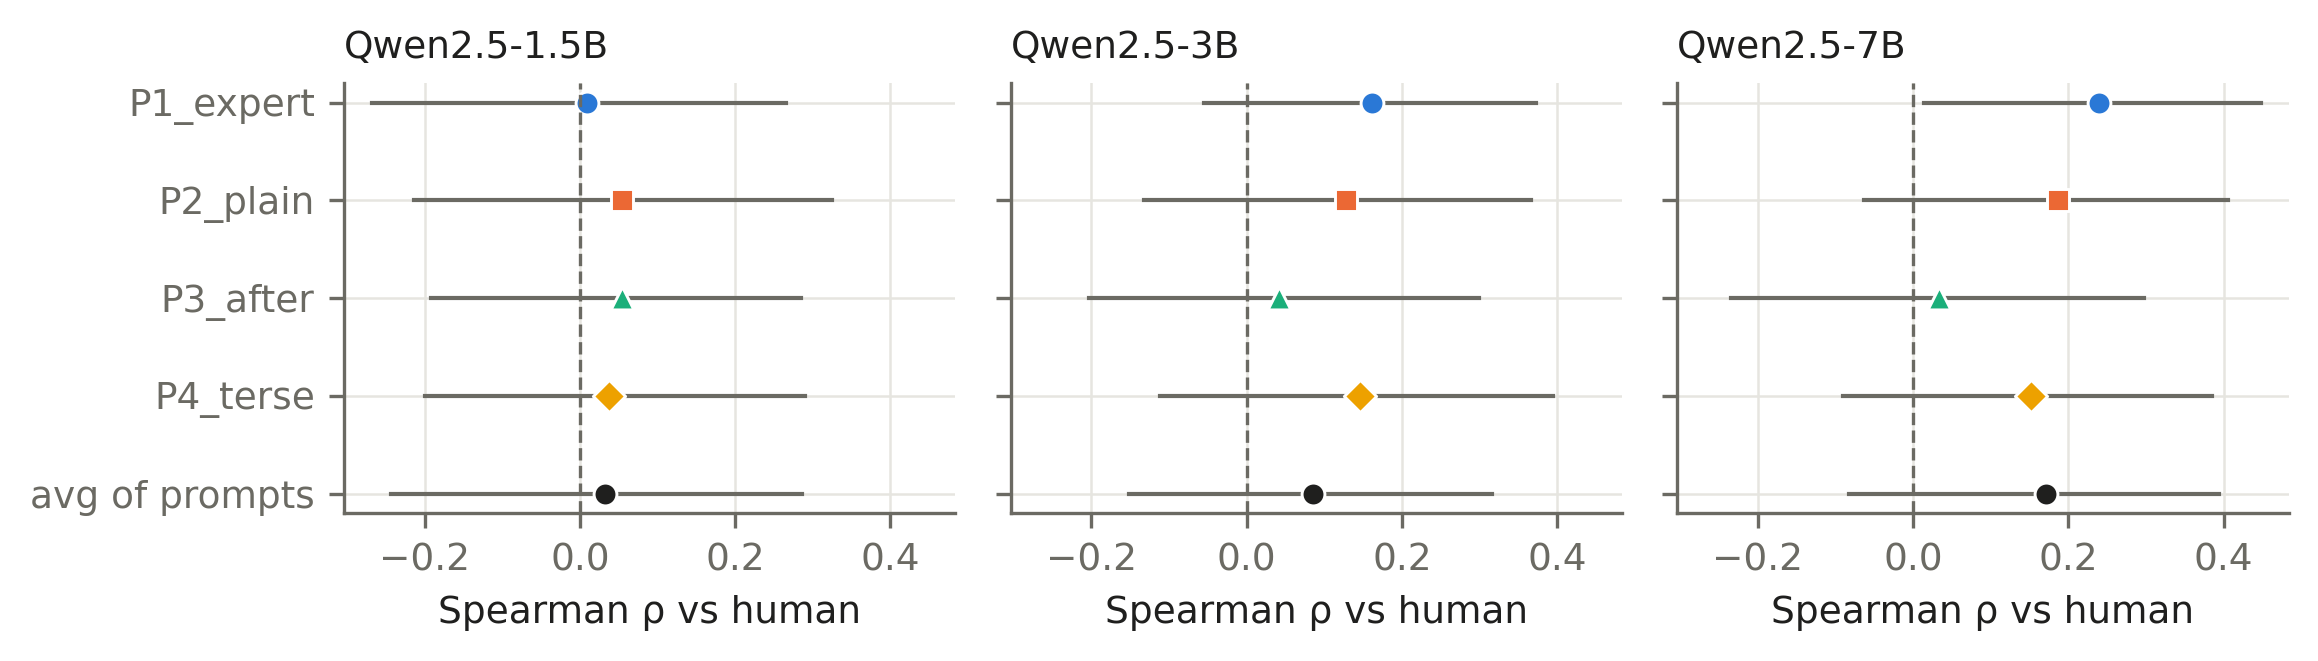
\includegraphics[width=\textwidth]{figures/fig2_agreement.png}
\caption{Correlation between model scores and human ratings for each prompt. Dots are the estimates, lines are 95\% confidence intervals, and the dashed line marks zero (no relationship). Nearly every line crosses zero.}
\label{fig:agreement}
\end{figure}

\subsection{Does averaging the prompts help?}
Averaging the scores from all four prompts gives results about as good as a typical single prompt, but not as good as the best one. Averaging is still the safer choice: you can only know which prompt is best after comparing against human ratings, and with a different set of papers a different prompt might come out on top.

\textbf{In short:} the models are fairly consistent with themselves but not with humans. Whatever they are using to rank papers, it is mostly not what human reviewers judge as quality.

% =====================================================================
\section{Limitations}
This is a small pilot study, and the results should be read with that in mind.
\begin{itemize}
  \item Only 60 papers, from one conference and one year, and only one family of models.
  \item The models saw only the title and abstract, not the full paper.
  \item ICLR 2024 papers and reviews may have been part of the models' training data.
  \item Human reviewers can only choose 1, 3, 5, 6, 8, or 10, while the finer model score can take any value, so some comparisons are approximate.
  \item With this many comparisons and only 60 papers, small differences between prompts or models may be due to chance.
\end{itemize}

% =====================================================================
\section{Conclusion}
Small open LLMs asked to review papers accept nearly everything, change a noticeable share of their verdicts when the prompt is reworded, and agree only weakly with human reviewers, although bigger models do somewhat better. Anyone using such a model as a reviewer should not rely on a single prompt: test several prompts that mean the same thing, and check the scores against human judgments before trusting them. Natural next steps are larger models, full papers instead of abstracts, other kinds of irrelevant changes (such as section order or length), and methods that make scores comparable across prompts.

\section*{Code and Data}
All code, prompts, model outputs, and analysis are available at \fillme{GitHub URL}.

\section*{Acknowledgments}
I used an AI assistant (Claude, by Anthropic) to help write code, run analyses, and draft and edit the text. I reviewed all of the content and take full responsibility for it.

% =====================================================================
\bibliographystyle{plainnat}
\bibliography{refs}

\clearpage
\appendix

\section{Full Prompt Text}
\label{app:prompts}
Each prompt was sent to the model as a single user message, exactly as shown below, including line breaks. The highlighted \slot{title} and \slot{abstract} are replaced with the paper's title and abstract.

\begin{promptbox}{P1 (expert) \hfill\normalfont\small Reviewer role, instructions first}
You are an expert reviewer for ICLR. Read the title and abstract below and rate the paper's overall quality on a scale from 1 (strong reject) to 10 (strong accept). Respond with a single integer only.\par
Title: \slot{title}\par
Abstract: \slot{abstract}
\end{promptbox}

\begin{promptbox}{P2 (plain) \hfill\normalfont\small Plain description, no role}
Below is a submission to the ICLR conference. As a reviewer, score it from 1 to 10, where 10 means a clear accept and 1 means a clear reject. Output just the number.\par
Title: \slot{title}\\
Abstract: \slot{abstract}
\end{promptbox}

\begin{promptbox}{P3 (after) \hfill\normalfont\small Instructions after the paper}
Title: \slot{title}\par
Abstract: \slot{abstract}\par
You are reviewing this paper for ICLR, a top machine learning conference. On a 1-10 scale (1 = strong reject, 10 = strong accept), what score would you give? Reply with one integer and nothing else.
\end{promptbox}

\begin{promptbox}{P4 (terse) \hfill\normalfont\small Short, markdown headings}
Rate this ICLR submission.\\
Scale: 1 (definitely reject) to 10 (definitely accept).\\
Format: a single integer.\par
\#\#\# Title\\
\slot{title}\par
\#\#\# Abstract\\
\slot{abstract}
\end{promptbox}

\section{Technical Details}
\label{app:details}

\textbf{Running the models.} The models are the instruction-tuned versions (\texttt{Qwen2.5-\{1.5B,\allowbreak 3B,\allowbreak 7B\}-\allowbreak Instruct}), run in 16-bit precision with deterministic (greedy) decoding and at most 8 new tokens. Every response contained a usable number.

\textbf{Finer score.} The finer score is the expected value of the model's answer,
\[
  \hat{s} = \sum_{s=1}^{10} s \cdot P(s \mid \text{prompt}),
\]
using the model's probabilities for its first output token, renormalized over the answers 1 to 10. Qwen writes numbers one digit at a time, so a first token of ``1'' could mean 1 or 10; I split it using the probability that the next token is ``0''. On average the models put at least 98\% of their probability on a numeric answer.

\textbf{Consistency measures.} Verdicts use the top 31\% of papers (19 of 60) under each prompt. With four prompts that ranked papers independently at random, the share of papers that flip would be $1 - 0.31^4 - 0.69^4 \approx 76\%$. The average change in a paper's finer score across prompts (standard deviation) was 0.19, 0.34, and 0.24 for the 1.5B, 3B, and 7B models; the lowest agreement between any two prompts' rankings was 0.65, 0.66, and 0.70.

\textbf{Statistics.} Correlations are Spearman rank correlations. Confidence intervals come from bootstrapping: resampling the 60 papers with replacement 1,000 times and taking the middle 95\% of results.

\end{document}
